\documentclass{article}

% packages
\usepackage{amsmath, amsthm, thmtools, amsfonts, amssymb, luacode, catchfile, tikzducks, hyperref, ifthen}
\ifcsname c@kobocompile\endcsname
	\usepackage[a5paper, total={1072pt, 1448pt}, margin=10pt, includeheadfoot]{geometry} % set page margins
\else
	\usepackage[a4paper, margin=50pt, includeheadfoot]{geometry}
\fi
\usepackage[shortlabels]{enumitem}
\usepackage[skip=3pt, indent=0pt]{parskip}

% language
\usepackage[bidi=basic, layout=tabular, provide=*]{babel}
\ifcsname c@english\endcsname
	\babelprovide[main, import]{english}
\else
	\babelprovide[main, import]{hebrew}
	\babelprovide{rl}
\fi
%\babelfont{rm}{Libertinus Serif}
\babelfont{rm}[Renderer=Harfbuzz]{Libertinus Serif}
\babelfont{sf}{Libertinus Sans}
\babelfont{tt}{Libertinus Mono}

% style
\AddToHook{cmd/section/before}{\clearpage}	% Add line break before section
\linespread{1.3}
\setcounter{secnumdepth}{0}		% Remove default number tags from sections, this won't do well with theorems
\AtBeginDocument{\setlength{\belowdisplayskip}{3pt}}
\AtBeginDocument{\setlength{\abovedisplayskip}{3pt}}
\graphicspath{ {../images/} }

% operators
\DeclareMathOperator\cis{cis}
\DeclareMathOperator\Sp{Sp}
\DeclareMathOperator\tr{tr}
\DeclareMathOperator\im{Im}
\DeclareMathOperator\re{Re}
\DeclareMathOperator\diag{diag}
\DeclareMathOperator*\lowlim{\underline{lim}}
\DeclareMathOperator*\uplim{\overline{lim}}
\DeclareMathOperator\rng{rng}
\DeclareMathOperator\Sym{Sym}
\DeclareMathOperator\Arg{Arg}
\DeclareMathOperator\Log{Log}
\DeclareMathOperator\dom{dom}
\DeclareMathOperator\supp{Supp}
\DeclareMathOperator\var{Var}
\DeclareMathOperator\cov{Cov}

% commands
%\renewcommand\qedsymbol{\textbf{מש''ל}}
%\renewcommand\qedsymbol{\fbox{\emoji{lizard}}}
\newcommand{\Aa}[0]{\mathcal{A}}
\newcommand{\Bb}[0]{\mathcal{B}}
\newcommand{\CC}[0]{\mathbb{C}}
\newcommand{\Cc}[0]{\mathcal{C}}
\newcommand{\EE}[0]{\mathbb{E}}
\newcommand{\FF}[0]{\mathbb{F}}
\newcommand{\Ff}[0]{\mathcal{F}}
\newcommand{\Ii}[0]{\mathcal{I}}
\newcommand{\Gg}[0]{\mathcal{G}}
\newcommand{\Ll}[0]{\mathcal{L}}
\newcommand{\Mm}[0]{\mathcal{M}}
\newcommand{\NN}[0]{\mathbb{N}}
\newcommand{\Nn}[0]{\mathcal{N}}
\newcommand{\PP}[0]{\mathbb{P}}
\newcommand{\Pp}[0]{\mathcal{P}}
\newcommand{\QQ}[0]{\mathbb{Q}}
\newcommand{\RR}[0]{\mathbb{R}}
\newcommand{\Rr}[0]{\mathcal{R}}
\newcommand{\Ss}[0]{\mathcal{S}}
\newcommand{\TT}[0]{\mathbb{T}}
\newcommand{\Uu}[0]{\mathcal{U}}
\newcommand{\Vv}[0]{\mathcal{V}}
\newcommand{\Ww}[0]{\mathcal{W}}
\newcommand{\ZZ}[0]{\mathbb{Z}}
\newcommand{\acts}[0]{\circlearrowright}
\newcommand{\explain}[2] {
	\begin{flalign*}
		 && \text{#2} && \text{#1}
	\end{flalign*}
}
\newcommand{\maketitleprint}[0]{ \begin{center}
	%\begin{tikzpicture}[scale=3]
	%	\duck[graduate=gray!20!black, tassel=red!70!black]
	%\end{tikzpicture}	
	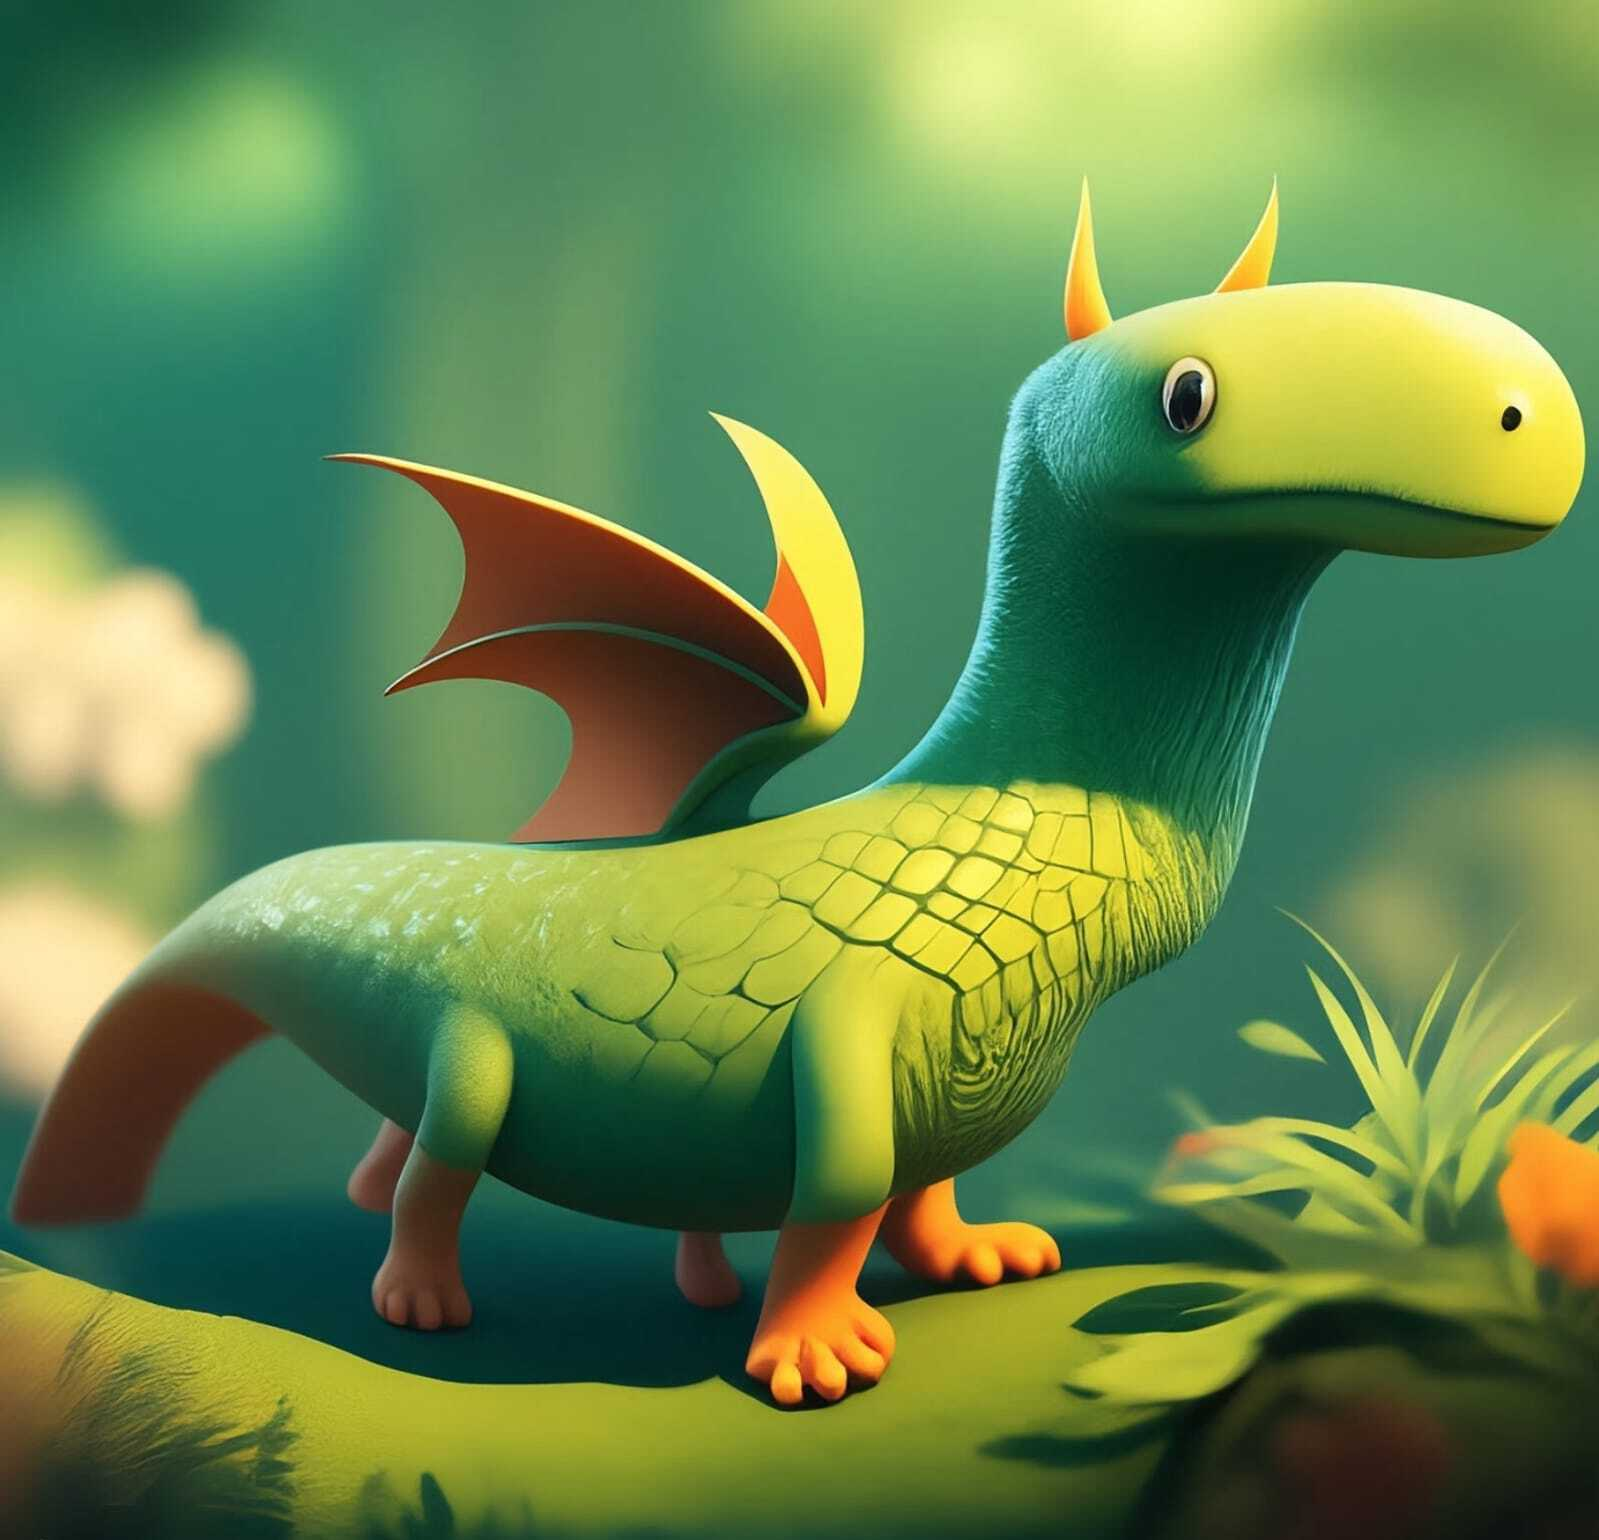
\includegraphics[width=6cm]{cover}
\end{center}
}

% theorem commands
\newtheoremstyle{c_remark}
	{}	% Space above
	{}	% Space below
	{}% Body font
	{}	% Indent amount
	{\bfseries}	% Theorem head font
	{}	% Punctuation after theorem head
	{.5em}	% Space after theorem head
	{\thmname{#1}\thmnumber{ #2}\thmnote{ \normalfont{\text{(#3)}}}}	% head content
\newtheoremstyle{c_definition}
	{3pt}	% Space above
	{3pt}	% Space below
	{}% Body font
	{}	% Indent amount
	{\bfseries}	% Theorem head font
	{}	% Punctuation after theorem head
	{.5em}	% Space after theorem head
	{\thmname{#1}\thmnumber{ #2}\thmnote{ \normalfont{\text{(#3)}}}}	% head content
\newtheoremstyle{c_plain}
	{3pt}	% Space above
	{3pt}	% Space below
	{\itshape}% Body font
	{}	% Indent amount
	{\bfseries}	% Theorem head font
	{}	% Punctuation after theorem head
	{.5em}	% Space after theorem head
	{\thmname{#1}\thmnumber{ #2}\thmnote{ \text{(#3)}}}	% head content

\ifcsname c@english\endcsname
	\theoremstyle{plain}
	\newtheorem{theorem}{Theorem}[section]
	\newtheorem{lemma}[theorem]{Lemma}
	\newtheorem{proposition}[theorem]{Proposition}
	\newtheorem*{proposition*}{Proposition}
	%\newtheorem{corollary}[theorem]{אין חלופה עברית}

	\theoremstyle{definition}
	\newtheorem{definition}[theorem]{Definition}
	\newtheorem*{definition*}{Definition}
	\newtheorem{example}{Example}[section]
	\newtheorem{exercise}{Exercise}[section]

	\theoremstyle{remark}
	\newtheorem*{remark}{Remark}
	\newtheorem*{solution}{Solution}
	\newtheorem{conclusion}[theorem]{Conclusion}
	\newtheorem{notation}[theorem]{Notation}
\else
	\theoremstyle{c_plain}
	\newtheorem{theorem}{משפט}[section]
	\newtheorem{lemma}[theorem]{למה}
	\newtheorem{proposition}[theorem]{טענה}
	\newtheorem*{proposition*}{טענה}
	%\newtheorem{corollary}[theorem]{אין חלופה עברית}

	\theoremstyle{c_definition}
	\newtheorem{definition}[theorem]{הגדרה}
	\newtheorem*{definition*}{הגדרה}
	\newtheorem{example}{דוגמה}[section]
	\newtheorem{exercise}{תרגיל}[section]

	\theoremstyle{c_remark}
	\newtheorem*{remark}{הערה}
	\newtheorem*{solution}{פתרון}
	\newtheorem{conclusion}[theorem]{מסקנה}
	\newtheorem{notation}[theorem]{סימון}
\fi

% Questions related commands
\newcounter{question}
\setcounter{question}{1}
\newcounter{sub_question}
\setcounter{sub_question}{1}

\ifcsname c@english\endcsname
	\newcommand{\question}[1][0]{
		\ifthenelse{#1 = 0}{}{\setcounter{question}{#1}}
		\section{Question \arabic{question}}
		\addtocounter{question}{1}
		\setcounter{sub_question}{1}
	}

	\newcommand{\subquestion}[1][0]{
		\ifthenelse{#1 = 0}{}{\setcounter{sub_question}{#1}}
		\subsection{Part \alph{sub_question}}
		\addtocounter{sub_question}{1}
	}
\else
	\newcommand{\question}[1][0]{
		\ifthenelse{#1 = 0}{}{\setcounter{question}{#1}}
		\section{שאלה \arabic{question}}
		\addtocounter{question}{1}
		\setcounter{sub_question}{1}
	}

	\newcommand{\subquestion}[1][0]{
		\ifthenelse{#1 = 0}{}{\setcounter{sub_question}{#1}}
		\subsection{סעיף \localecounter{letters.gershayim}{sub_question}}
		\addtocounter{sub_question}{1}
	}
\fi

% import lua and start of document
\directlua{common = require ('../common')}

\GetEnv{AUTHOR}

% headers
\author{\AUTHOR}
\date\today

\title{פתרון מטלה 10 --- מבוא ללוגיקה, 80423}

\begin{document}
\maketitle
\maketitleprint{}

\question{}
ניזכר בהוכחה מהתרגול, ובפרט בענף $b$ מההוכחה האחרונה.

\subquestion{}
נוכיח ש־$b$ הוא קבוצת הינטיקה הכוללת את $\Sigma \cup \{ \lnot \varphi \}$.
\begin{proof}
	נתון לנו כי $\Pi$ חסכונית, וכן מהגדרת $f$ והענף $b$ אנו יודעים (הוכח בתרגול) שלכל $\psi \in \Pi \implies \psi \in b$, ולכן נשתמש בתכונות קבוצה חסכונית כדי להוכיח ש־$b$ קבוצת הינטיקה.
	כהערה, בתרגיל הקודם מספרנו את התכונות של קבוצת הינטיקה לצורך קריאות ההוכחה, מספור זה הוא לפי הסדר בו התנאים מופיעים בתרגיל הקודם.
	\begin{enumerate}
		\item אם $P$ פסוק יסודי אז מהגדרת הרקורסיה אין סתירה בענף ולכן $\lnot P \notin b$.
		\item אם $\psi_1 \land \psi_2 \in \Pi$ אז מהגדרת חסכונית $\psi_1, \psi_2 \in \Pi$, באופן דומה אם $\lnot (\psi_1 \land \psi_2) \in \Pi$ אז שלילת אחד הפסוקים ב־$\Pi$, ואנו עומדים בהגדרה של קבוצת הינטיקה לגימום.
		\item אם $\psi_1 \lor \psi_2 \in \Pi$ אז מהעובדה שבענף אין סתירות נובע ש־$\psi_1 \in b$ או $\psi_2 \in b$ כפי שרצינו.
			אם $\lnot (\psi_1 \lor \psi_2) \in \Pi$ אז $\psi_1 \lor \psi_2 \in \Pi$ ולכן בשל החוסר בסתירות $\lnot \psi_1 \in b$ ואנו עומדים בהגדרה.
		\item אם $\psi_1 \to \psi_2 \in \Pi$ אז $\psi_1 \in \Pi$ ולכן גם $\psi_2 \in b$, אם $\lnot (\psi_1 \to \psi_2) \in \Pi$ אז $\psi_1 \to \psi_2 \in \Pi$ ומחוסר הסתירות ב־$b$ גם $\psi_1, \lnot \psi_2 \in b$.
		\item אם $\psi_1 \leftrightarrow \psi_2 \in \Pi$ אז $\psi_1, \psi_2, \lnot \psi_1, \lnot \psi_2 \in \Pi$ ומחוסר הסתירות $\psi_1, \psi_2 \in b$ או $\lnot \psi_1, \lnot \psi_2 \in b$ בהתאם להגדרה.
			אם שלילת הגרירה הדו־כיוונית ב־$\Pi$ אז באופן דומה נקבל את התנאי עבור $\psi_1, \lnot \psi_2$ או $\lnot \psi_1, \psi_2$
			אם שלילת הגרירה הדו־כיוונית ב־$\Pi$ אז באופן דומה נקבל את התנאי עבור $\psi_1, \lnot \psi_2$ או $\lnot \psi_1, \psi_2$.
	\end{enumerate}
	בהתאם מצאנו כי כל התנאים של קבוצת הינטיקה נובעים מההגדרה של קבוצה חסכונית יחד עם העובדה ש־$b$ ענף ללא סתירות (שאם לא כן הוא לא הייתה הצדקה להגדרתו). \\
	נבחין ש־$\lnot \varphi \in b$ מההגדרה של הענף, וכן בתרגול הנחנו $\sigma \cup \{ \lnot \varphi \} \subseteq \Pi$ ולכן כמובן $\Sigma \subseteq b$.
\end{proof}

\subquestion{}
נסיק שלכל $\Pi$ חסכונית, $\varphi$ ו־$\Sigma$, כך ש־$\Sigma \cup \{ \varphi \} \subseteq \Pi$ ו־$\Sigma \models \varphi$ קיים עץ היסק של $\varphi$ מ־$\Sigma$ המכיל רק פסוקים מ־$\Pi$.
\begin{proof}
	נשתמש בהוכחה מהתרגול ונקבל שאו שיש עץ היסק סופי המקיים את התנאי המבוקש, או שבעץ היסק זה יש ענף אינסופי $b$ כפי שתואר בתרגול. \\
	ענף זה כפי שראינו זה עתה הוא קבוצת הינטיקה ולכן לפי שאלה 1 של המטלה הקודמת הוא ספיק, כלומר קיים $v : L \to \{ \TT, \FF \}$ כך ש־$\forall \psi \in b, \bar{v}(\psi) = \TT$.
	אבל $\varphi$ הערכת אמת שמספקת את $\Sigma$, ונתון שבמקרה זה $\bar{v}(\varphi) = \TT$, אבל $\lnot \varphi \in b$ ולכן גם $\bar{v}(\lnot \varphi) = \TT$, כלומר הגענו לסתירה, וענף זה בהכרח מכיל סתירה. \\
	בשל הופעת הפסוק נוכל בפרט לקבל סתירה לאינסופיות, כלומר קיבלנו עץ היסק שבו יש סתירה בכל ענף וגם כל ענף הוא סופי כפי שרצינו.
\end{proof}

\question{}
תהי $L$ שפה לתחשיב יחסים.

\subquestion{}
נראה שאם $\varphi$ פסוק אז לכל משתנה $x$ מתקיים $\forall x \varphi \vdash \varphi$.
\begin{proof}
	נבחין ש־$x$ איננו משתנה חופשי ב־$\varphi$ שכן $\varphi$ פסוק, לכן נוכל לקבוע ש־$\varphi_t^x = \varphi$ לכל $t \in \operatorname{term}_L$. \\
	בהתאם נוכל לבנות את עץ ההיסק הבא
	\begin{enumerate}
		\item $\lnot \varphi$
		\item $\forall x \varphi$, הוספת הנחה
		\item $\varphi_c^x$, הצבה עבור קבוע כלשהו $c$
		\item $\varphi$, כלל החזרה, שימוש בזהות שמצאנו זה עתה, וסתירה
	\end{enumerate}
	ולכן $\forall x \varphi \vdash \varphi$.
\end{proof}

\subquestion{}
נניח ש־$L'$ שפה המתקבלת מ־$L$ על־ידי הוספת סימני קבוע מכמות כלשהי $\le \omega$. \\
נניח ש־$\Sigma$ תורה ב־$L$ וש־$\varphi$ פסוק ב־$L$.
נסמן $\Sigma \vdash_{L'} \varphi$ כאשר יש עץ היסק של $\varphi$ מ־$\Sigma$ ב־$L'$. \\
נראה שאם $\Sigma \vdash_{L'} \varphi$ אז $\Sigma \vdash_L \varphi$.
\begin{proof}
	נניח שבעץ ההיסק שמעיד על $\Sigma \vdash_{L'} \varphi$ ישנה הופעה של קבוצת הפסוקים $C = \{ c_i \mid i \le \alpha < \omega \} \subseteq \operatorname{const}_{L'} \setminus \operatorname{const}_L$. \\
	נעיר ש־$C$ קבוצה סופית, אחרת עץ ההיסק עצמו לא סופי בסתירה להגדרתו.
	נבחין כי מסופיות הפסוק ועץ ההיסק, $|C| < \omega$, ולכן נוכל לבצע תהליך אינדוקטיבי על־ידי שימוש במשפט ההכללה על־ידי פסוקים ולהסיק שגם $\Sigma \vdash_{L'} \forall c_1 \dots \forall c_\alpha \varphi$.
	מהמשפט $c_i$ לא מופיע בעץ ההיסק המעיד על כך לכל $i \le \alpha$, ולכן עץ היסק זה מעיד גם על $\Sigma \vdash_L \forall c_1 \dots \forall c_\alpha \varphi$.
	נוכל אם כן להשתמש בסעיף א' כדי לבצע עוד תהליך אינדוקטיבי שיניב לנו את הטענה $\Sigma \vdash_L \varphi$ כפי שרצינו.
\end{proof}

\subquestion{}
נסיק שאם $\Sigma$ עקבית כתורה ב־$L$ אז היא עקבית כתורה ב־$L'$.
\begin{proof}
	אילו נניח ש־$\Sigma$ לא עקבית כתורה ב־$L'$ אז $\Sigma \vdash_{L'} \perp$.
	אבל מסעיף ב' נובע ישירות ש־$\Sigma \vdash_L \perp$ בסתירה לעקביות $\Sigma$ תחת $L$.
\end{proof}

\question{}
תהי $\Sigma$ קבוצת פסוקים ב־$L$. \\
נגדיר $E \subseteq \operatorname{form}_L^2$ על־ידי
\[
	\alpha E \beta \iff \Sigma \vdash \alpha \leftrightarrow \beta
\]
נראה ש־$E$ יחס שקילות.
\begin{proof}
	נבחן את כלל התכונות של יחס שקילות.

	עבור רפלקסיביות, נבנה את עץ ההיסק הבא
	\begin{enumerate}
		\item $\lnot (\alpha \leftrightarrow \alpha)$
		\item פיצול למקרים על $\alpha$
			\begin{enumerate}
				\item $\alpha$
				\item $\lnot \alpha$, כללי גרירה דו־כיוונית מ־1, וסתירה
			\end{enumerate}
			\begin{enumerate}
				\item $\lnot \alpha$
				\item $\alpha$, כללי גרירה דו־כיוונית מ־1, וסתירה
			\end{enumerate}
	\end{enumerate}
	ולכן $\vdash \alpha \leftrightarrow \alpha$ ובפרט $\Sigma \vdash \alpha \leftrightarrow \alpha$ ואכן $\forall \alpha \in \operatorname{form}_L, \alpha E \alpha$.

	עבור סימטריה נניח ש־$\alpha, \beta \in \dom E$ כך ש־$\alpha E \beta$, לכן $\Sigma \vdash \alpha \leftrightarrow \beta$. \\
	בנוסף נבנה עץ היסק ל־$\Sigma \cup \{ \alpha \leftrightarrow \beta \} \vdash \beta \leftrightarrow \alpha$:
	\begin{enumerate}
		\item $\lnot (\beta \leftrightarrow \alpha)$
		\item $\alpha \leftrightarrow \beta$, הוספת הנחה
		\item פיצול למקרים על $\alpha$
			\begin{enumerate}
				\item $\alpha$
				\item $\beta$, חוקי גרירה דו־כיוונית ל־2
				\item $\lnot \beta$, חוקי גרירה דו־כיוונית ל־1, וסתירה
			\end{enumerate}
			\begin{enumerate}
				\item $\lnot \alpha$
				\item $\lnot \beta$, חוקי גרירה דו־כיוונית ל־2
				\item $\beta$, חוקי גרירה דו־כיוונית ל־1, וסתירה
			\end{enumerate}
	\end{enumerate}
	ולכן מטרנזיטיביות ההיסק נובע $\Sigma \vdash \beta \leftrightarrow \alpha$ וכן $\alpha E \beta \implies \beta E \alpha$.

	עבור טרנזיטיביות נניח ש־$\alpha E \beta, \beta E \gamma$ ונראה ש־$\Sigma \cup \{ \alpha \leftrightarrow \beta, \beta \leftrightarrow \gamma \} \vdash \alpha \leftrightarrow \gamma$,
	\begin{enumerate}
		\item $\lnot (\alpha \leftrightarrow \gamma)$
		\item $\alpha \leftrightarrow \beta$, הוספת הנחה
		\item $\beta \leftrightarrow \gamma$, הוספת הנחה
		\item פיצול למקרים על $\alpha$
			\begin{enumerate}
				\item $\alpha$
				\item $\beta$, כללי גרירה דו־כיוונית ל־2
				\item $\gamma$, כללי גרירה דו־כיוונית ל־3
				\item $\lnot \gamma$, כללי גרירה דו־כיוונית ל־1, וסתירה
			\end{enumerate}
			\begin{enumerate}
				\item $\lnot \alpha$
				\item $\lnot \beta$, כללי גרירה דו־כיוונית ל־2
				\item $\lnot \gamma$, כללי גרירה דו־כיוונית ל־3
				\item $\gamma$, כללי גרירה דו־כיוונית ל־1, וסתירה
			\end{enumerate}
	\end{enumerate}
	ולכן מטרנזיטיביות ההיסק $\Sigma \vdash \alpha \leftrightarrow \gamma$ וכן $\alpha E \gamma$ כפי רצינו להראות, ו־$E$ אכן יחס שקילות.
\end{proof}

\question{}
\subquestion{}
נוכיח שאין פסוק ב־$L_=$ כך ש־$\Aa$ מבנה ל־$L_=$ מספקת אותו אם ורק אם היא סופית.
\begin{proof}
	נניח בשלילה שקיים פסוק $\varphi$ כך ש־$\Aa \models \varphi \iff |A| < \omega$. \\
	ניזכר ב־$\varphi_{\ge n}$ שהגדרנו במטלות הקודמות ומקיים $\Aa \models \varphi_{\ge n} \iff |A| \ge n$,
	ונגדיר $\Sigma = \{ \varphi \} \cup \{ \varphi_{\ge n} \mid n < \omega \}$.
	עתה נראה ש־$\Sigma$ ספיקה סופית. תהי $\Pi \subseteq \Sigma$ כך ש־$|\Pi| < \omega$ ו־$n = \sup \{ n < \omega \mid \varphi_{\ge n} \in \Pi \}$, אז $\Bb = \langle [n + 1]; = \rangle$ מודל כך ש־$\Bb \models \Pi$ לפי בדיקה.
	בנוסף $\Bb$ מודל סופי ולכן $\Bb \models \varphi$.
	אז $\Sigma$ ספיקה סופית ולכן ממשפט הקומפקטיות ספיקה, לכן קיים מודל $\Aa \models \Sigma$, אבל $|A| \ge n$ לכל $n < \omega$, לכן $|A| \ge \omega$ ובפרט $\Aa \not\models \varphi$ בסתירה ל־$\Aa \models \varphi$.
	לכן לא קיים פסוק $\varphi$ כזה.
\end{proof}

\subquestion{}
יהי $\Gg = \langle V, E \rangle$ גרף.
נגדיר $\forall v, u \in V, S_{v, u} = \{ \langle v_0, \dots, v_{n - 1} \rangle \mid v_0 = v, v_{n - 1} = u, \langle v_0, \dots, v_{n - 1} \rangle \in V^n, n < \delta \}$, \\
בשאלה זו נניח $\delta = \omega$, וכן $d(v, u) = \inf_{s \in S_{v, u}} |s|$ ונסמן $d(v, u) = \infty$ אם $S_{u, v} = \emptyset$.
נגדיר את הקוטר של $\Gg$ להיות $D(\Gg) = \min \{ n \mid \forall v, u \in V, d(v, u) \le n \}$. \\
תהי $L = \{ E \}$ עבור $E$ סימן יחס דו־מקומי, ונוכיח שלכל $n < \omega$ קיים פסוק $\varphi_{D > n}$ כך ש־$\Gg \models \varphi_{D > n} \iff D(\Gg) > n$.
\begin{proof}
	נגדיר
	\[
		\varphi_{D > n}
		= \lnot (\forall v \forall u (\exists v_0 \dots \exists v_{n - 1} (v = v_0 \land u = v_{n - 1} \land E(v_0, v_1) \land \cdots \land E(v_{n - 2}, v_{n - 1}))))
	\]
	ונראה שאכן $\Gg \models \varphi_{D > n} \iff D(\Gg) > n$.

	נניח ש־$\Gg \models \varphi_{D > n}$ ולכן מהגדרת הפסוק נובע ישירות שקיימים שני קודקודים ב־$V$ כך שאין ביניהם מסלול באורך $n$, ולכן אין ביניהם גם מסלול קטן מ־$n$ (אחרת היינו יכולים להגדיל אותו באופן טריוויאלי).
	לכן לפי ההגדרה $D(\Gg) > n$. \\
	מהכיוון השני אם נניח ש־$D(\Gg) > n$ אז $d(v, u) > n$ לכל $v, u \in V$, ובפרט לא קיים מסלול באורך $n$ בין קודקודים אלה, וזהו תוכן הפסוק במדויק.
\end{proof}

\subquestion{}
נסיק מהסעיף הקודם שאין פסוק $\varphi$ ב־$L$ כך ש־$\Gg \models \varphi \iff D(\Gg) < \infty$.
\begin{proof}
	נניח בשלילה שקיים $\varphi$ פסוק כך ש־$\Gg \models \varphi \iff D(\Gg) < \infty$, ונגדיר $\Sigma = \{ \varphi \} \cup \{ \varphi_{D < n} \mid n < \omega \}$.
	לכל $\Pi \subseteq \Sigma$ כך ש־$|\Pi| < \omega$, נגדיר $\Gg = \langle [n + 1], \{ \{i, i + 1\} \mid i < n + 1 \} \rangle$ גרף כך ש־$D(\Gg) = n + 1$ עבור $n = \sup \{ n \mid \varphi_{D > n} \in \Pi \}$.
	בהתאם $\Gg \models \Pi$, שהרי המסלול בין $0$ ו־$n$ הוא באורך של $n$ לכל הפחות. בפרט $\Gg \models \varphi$ שכן הוא סופי.
	כמו בסעיף א' נובע ממשפט הקומפקטיות שקיים $\Gg \models \Sigma$, אבל בהתאם נובע עבור ה־$n$ שהגדרנו ש־$n = \omega$, כלומר $D(\Gg) = \infty$, ולכן $\Gg \not\models \varphi$ בסתירה ל־$\Gg \models \Sigma \ni \varphi$.
\end{proof}

\question{}
נוכיח שאין פסוק ב־$L = \{ E \}$ שהגדרנו בשאלה 4 כך שגרף $\Gg$ מקיים $\Gg \models \varphi \iff \forall u, v \in V, d(u, v) < \infty$.
\begin{proof}
	נניח בשלילה שיש פסוק כזה, $\varphi$, ונגדיר את קבוצת הפסוקים, $\Sigma = \{ \varphi \} \cup \{ \varphi_{D > n} \mid n < \omega \}$.
	לכל $\Pi \subseteq \Sigma$ כך ש־$|\Pi| < \omega$ נגדיר $n = \max\{ n \mid \varphi_{D > n} \in \Pi \}$, ובהתאם נגדיר $\Gg_n = \langle [n + 1], \{ \{n, n + 1\} \mid n \in [n] \}\rangle$.
	נבחין ש־$\Gg_n \models \varphi_{D > m}$ לכל $m < n$, וכן כמובן מהסופיות וההנחה $\Gg_n \models \varphi$, לכן $\Gg_n \models \Pi$.
	כל $\Pi$ ספיקה ולכן $\Sigma$ ספיקה סופית ולכן מקומפקטיות ספיקה, לכן יהי $\Gg \models \Sigma$.
	אנו יודעים ש־$\Gg \models \varphi$ ולכן יהיו $u, v \in V$ כך שמרחקם מקסימלי, נבחין שלכל $n < \omega$ גם $\Gg \models \varphi_{D > n}$ ולכן מהגדרתם $d(u, v) > n$, לכן נוכל להסיק $d(u, v) = \sup n = \omega$.
	זוהי כמובן סתירה לסופיות כלל המסלולים, לכן נוכל להסיק שאין פסוק $\varphi$ כזה.

	אנסה לפתור את השאלה בדרך שאיננה חלק מהחומר ואשמח לביקורת,
	נניח ש־$\kappa$ מונה קומפקטי חזק (strongly compact) ונניח עתה שאנו עובדים מעל $\Ll_{\kappa, \kappa}(L)$, ונגדיר את השאלה מחדש.
	נגדיר $\Gg \models \varphi \iff \forall u, v \in V, d(u, v) < \kappa$.
	בשאלה זו נניח $\delta = \kappa$, כלומר אנו מגדירים מסלולים באופן מורחב. \\
	נגדיר את הפסוק $\varphi_\alpha = \exists u, v (\exists_{i < \alpha} v_i ((\bigwedge_{i < j < \alpha} \lnot (v_i = v_j)) \land (\bigwedge_{i + 1 < \alpha} E(v_i, v_{i + 1}))))$ לכל $\alpha < \kappa$. \\
	נגדיר $\Sigma_\alpha = \{ \varphi \} \cup \{ \varphi_\beta \mid n < \beta \}$,
	ולכן אם נגדיר $\Gg_\alpha = \langle \alpha + 1; \{ \{ v_\gamma, v_{\gamma + 1} \} \mid \gamma < \alpha \} \rangle$ ינבע $\Gg_\alpha \models \Sigma_\alpha$ לכל $\alpha < \kappa$.
	מהקומפקטיות החזקה של $\kappa$ חל על קבוצה זו ולכן הקבוצה $\Sigma_\lambda$ ספיקה ומסופקת על־ידי $\Gg_\kappa$, אבל $\Gg_\omega \models \varphi_\kappa$, בסתירה ל־$\varphi$. \\
	במקרה הפרטי של $\kappa = \omega$ נקבל את השאלה המקורית, ושם נשתמש במשפט הקומפקטיות כדי לקבל את מבוקשנו.
\end{proof}

\end{document}
